\documentclass[11pt,a4paper]{article}

\usepackage{geometry}
 \geometry{
 a4paper,
 total={150mm,237mm},
 left=30mm,
 top=30mm,
 }

% cf. http://tex.stackexchange.com/questions/50182/subtitle-with-the-maketitle-page
\usepackage{titling}
\newcommand{\subtitle}[1]{%
  \posttitle{%
    \par\end{center}
    \begin{center}\large\textbf{#1}\end{center}
    \vskip0.5em}%
}

\usepackage{color}
\usepackage{graphicx}
\usepackage[pdftex,colorlinks=false]{hyperref}
% get rid of the horrible coloured boxes around links
\hypersetup{
    colorlinks,%
    citecolor=black,%
    filecolor=black,%
    linkcolor=black,%
    urlcolor=black
}

\usepackage[UKenglish,german]{babel}

\usepackage{fancyvrb}
\VerbatimFootnotes

\widowpenalty10000  % http://tex.stackexchange.com/questions/4152/how-do-i-prevent-widow-orphan-lines
\clubpenalty10000

\title{The SysSon Platform}
\subtitle{Technical Report TR-2016-08-1\\Institute of Electronic Music and Acoustics, Graz}
\author{Hanns Holger Rutz}
% \date{09-Feb-2016}
\date{August 2016}

% \renewcommand*\rmdefault{dayrom}
% \usepackage{concmath}
\usepackage[lf]{venturis} %% lf option gives lining figures as default; 
			  %% remove option to get oldstyle figures as default
% \renewcommand*\familydefault{\sfdefault} %% Only if the base font of the document is to be sans serif
\usepackage[T1]{fontenc}

% cf. https://tex.stackexchange.com/questions/94126/change-font-to-only-section-and-subsection-of-my-document
%\usepackage{titlesec}
%\titleformat{\chapter}[display]
%  {\fontfamily{pag}\selectfont\huge\bfseries}
%  {\chaptertitlename\ \thechapter}
%  {20pt}
%  {\Huge}
%\titleformat{\section}
%  {\fontfamily{pag}\selectfont\bfseries\Large}
%  {\thesection}
%  {1em}
%  {}
%\titleformat{\subsection}
%  {\fontfamily{pag}\selectfont\bfseries\Large}
%  {\thesection}
%  {1em}
%  {}


\usepackage[utf8]{inputenc}
%\usepackage[backend=biber,natbib=true,citestyle=verbose-ibid,isbn=false,maxnames=3,bibstyle=authoryear,useprefix=true,sorting=ydnt]{biblatex} % citereset=chapter
\usepackage[backend=biber,natbib=true,citestyle=verbose-ibid,isbn=false,maxnames=20,bibstyle=authoryear,firstinits=true,sorting=ydnt,useprefix=true]{biblatex} % citereset=chapter, 
\addbibresource{rutz.bib} % add a bib-reference file

% warning: https://tex.stackexchange.com/questions/313477/
% \usepackage{csquotes}

\usepackage{tabularx}
% cf. https://tex.stackexchange.com/questions/84400/table-layout-with-tabularx-column-widths-502525
\newcolumntype{s}{>{\hsize=1cm}X}

% says you should load after babel and fontspec
\usepackage[shrink=10, babel=true]{microtype}	% http://tex.stackexchange.com/questions/141852/latex-allows-line-break-between-concluding-em-dash-and-comma-before-a-new-sub-cl/141854#141854

\newcommand{\todo}[1]{\colorbox{yellow}{\textsc{todo}: #1}}

\newcommand{\quot}[1]{\guillemotleft {#1}\guillemotright}

\newcommand{\worktitle}[1]{\textit{#1}}

\newcommand{\workentry}[2]{\vspace{7.5pt}\noindent\textbf{#1} (#2)}
\newcommand{\workentrySel}[2]{\vspace{7.5pt}\noindent\textbf{#1}$*$ (#2)}

\newcommand{\figref}[1]{Fig.~\ref{#1}}

\newcommand{\software}[1]{\textit{#1}}

\newcommand{\sysson}[0]{SysSon}
\newcommand{\syssonVersion}[0]{1.8.0}
\newcommand{\syssonVersionS}[0]{1.8.0-SNAPSHOT}

\begin{document}
% \begin{titlepage}
\maketitle
\selectlanguage{UKenglish}
\thispagestyle{empty}
\newpage
\section{\todo{}}

\subsection{Libraries and Modules}

\sysson{} is built with the \software{sbt} build tool.\footnote{\url{http://www.scala-sbt.org/}} \software{Sbt} manages module and library dependencies though a software called \software{Ivy} and using so-called \software{Maven} artefacts. Such artefacts are composed of a group-identifier, artefact-identifier, and a version string. For example, \sysson{} itself has group-id \verb!at.iem.sysson!, artefact-id \verb!sysson!, and current version \verb!1.8.0-SNAPSHOT!. The version scheme is the one proposed as \emph{Semantic Versioning}\footnote{\url{http://semver.org/}}, i.e. \verb!MAJOR.MINOR.PATCH!. The \verb!MAJOR! version indicates an entire new architecture, where the first stable generation is usually indicated by the digit \verb!1!. The \verb!MINOR! version indicates incremental changes, while the \verb!PATCH! version indicate bug fixes without change in functionality. In the Scala eco-system, the terminology is slightly different, where the major version is called "epoch", the minor version is called major version and the patch version is called minor version. So Scala 2.11.8, the latest release, has epoch 2, major version 11, and minor version 8 in the Scala terminology. We will henceforth use this naming scheme. The special suffix \verb!-SNAPSHOT! indicates that the version is not a stable released artefact but work in progress. Stable artefacts of libraries are published to a repository such a the public Maven Central,\footnote{\url{http://central.sonatype.org/}} and build tools can thus automatically download required artefacts based on a description of an application's dependencies.

The Maven based build tool \software{sbt} assumes a \emph{binary compatibility} between all minor versions, whereas the major version must be incremented when a binary incompatible change is introduced. A binary incompatibility means that the Java byte code of the library contains changes that make it unsafe for use with a caller that was compiled against a different version. This happens for example if a method has been removed from public API or changed in signature. Sbt automatically chooses the highest minor version if there are several transitive dependencies on the same artefact but with different minor versions, while it warns when transitive dependencies exist for the same artefact with different major versions. This also applies to the Scala version a library was compiled against, meaning that a binary file resulting from compilation against Scala 2.10.x (where x is any minor version) is binary incompatible with a binary file resulting from compilation against Scala 2.11.x (with 2.11.8 being the currently most recent release version). To ease this difficulty, sbt has introduced a mechanism called cross-versioning. Often Scala releases are still source compatible, and thus it is possible, for example, to compile the same source code against Scala 2.10.x and 2.11.x without changes. The artefacts will then be ``tagged'' by appending the major Scala version, e.g. the artifact-id becomes \verb!sysson_2.11! when compiling against Scala 2.11.x (this is independent of the regular Maven version).

This versioning scheme can be observed in the dependency graph that shows all the libraries and transitive libraries,\footnote{Transitive means a library A is used by another library B, and B is used by \sysson{}. Then A is a transitive dependency of \sysson{}.} generated by the \software{sbt-dependency-graph} plugin\footnote{The call is \verb!sbt dependencyDot!.} and shown in \figref{fig:dependencies}.\footnote{In the figure, lower level transitive third-party dependencies have been omitted for a clearer overview.} We can see the \sysson{} main artefact on the left-hand side with arrows pointing to immediate dependencies (libraries), which in turn point to other transitive libraries. Some libraries are published as a set of related artefacts, often bound together by one ``virtual'' meta-package. For example, the \software{Mellite} computer music environment is actually composed of two artefacts \verb!mellite-core! and \verb!mellite-views!, combined as virtual artefact \verb!mellite!. The \verb!-views! artefact connects to the graphical user interface, whereas \verb!-core! only contains data structures. Since \verb!-views! depends on \verb!-core! but not vice versa, it means we can develop a library merely based on the data structures without requiring the dependency on any GUI.

\subsubsection{Licensing Questions}

This approach helps keeping the code base modular, and furthermore can improve the licensing situation: In general we try to avoid dependency on GPL licensed code,\footnote{\url{https://www.gnu.org/licenses/gpl.html}} because it enforces the GPL on the entire product, something that is not the case with the LGPL\footnote{\url{https://www.gnu.org/copyleft/lesser.html}} or even more permissive licenses. We try to decouple GPL dependencies as far as possible, allowing for LGPL terms in most cases. GPL artefacts are often commercially developed products, because a commercial client company will likely not want to release their own product as open source under GPL terms and is thus forced to buy a commercial license from the library vendor, an approach that is called dual licensing. For example, the \software{iText} PDF library is available for free under GPL terms or by buying a commercial license that allows the client to develop their product without requiring to open source it. The same is true for the \software{Berkeley DB} database (developed by Oracle) and the \software{WebLaF} user interface look-and-feel. We currently do not own any commercially bought licenses, and thus \textbf{\sysson{} must be licensed under GPL version 3} terms. However except for the mentioned GPL based libraries, we have control over most other libraries, and thus in the future a different license might be chosen if replacements are found for the GPL libraries (or commercial licenses purchased).

\begin{figure}%
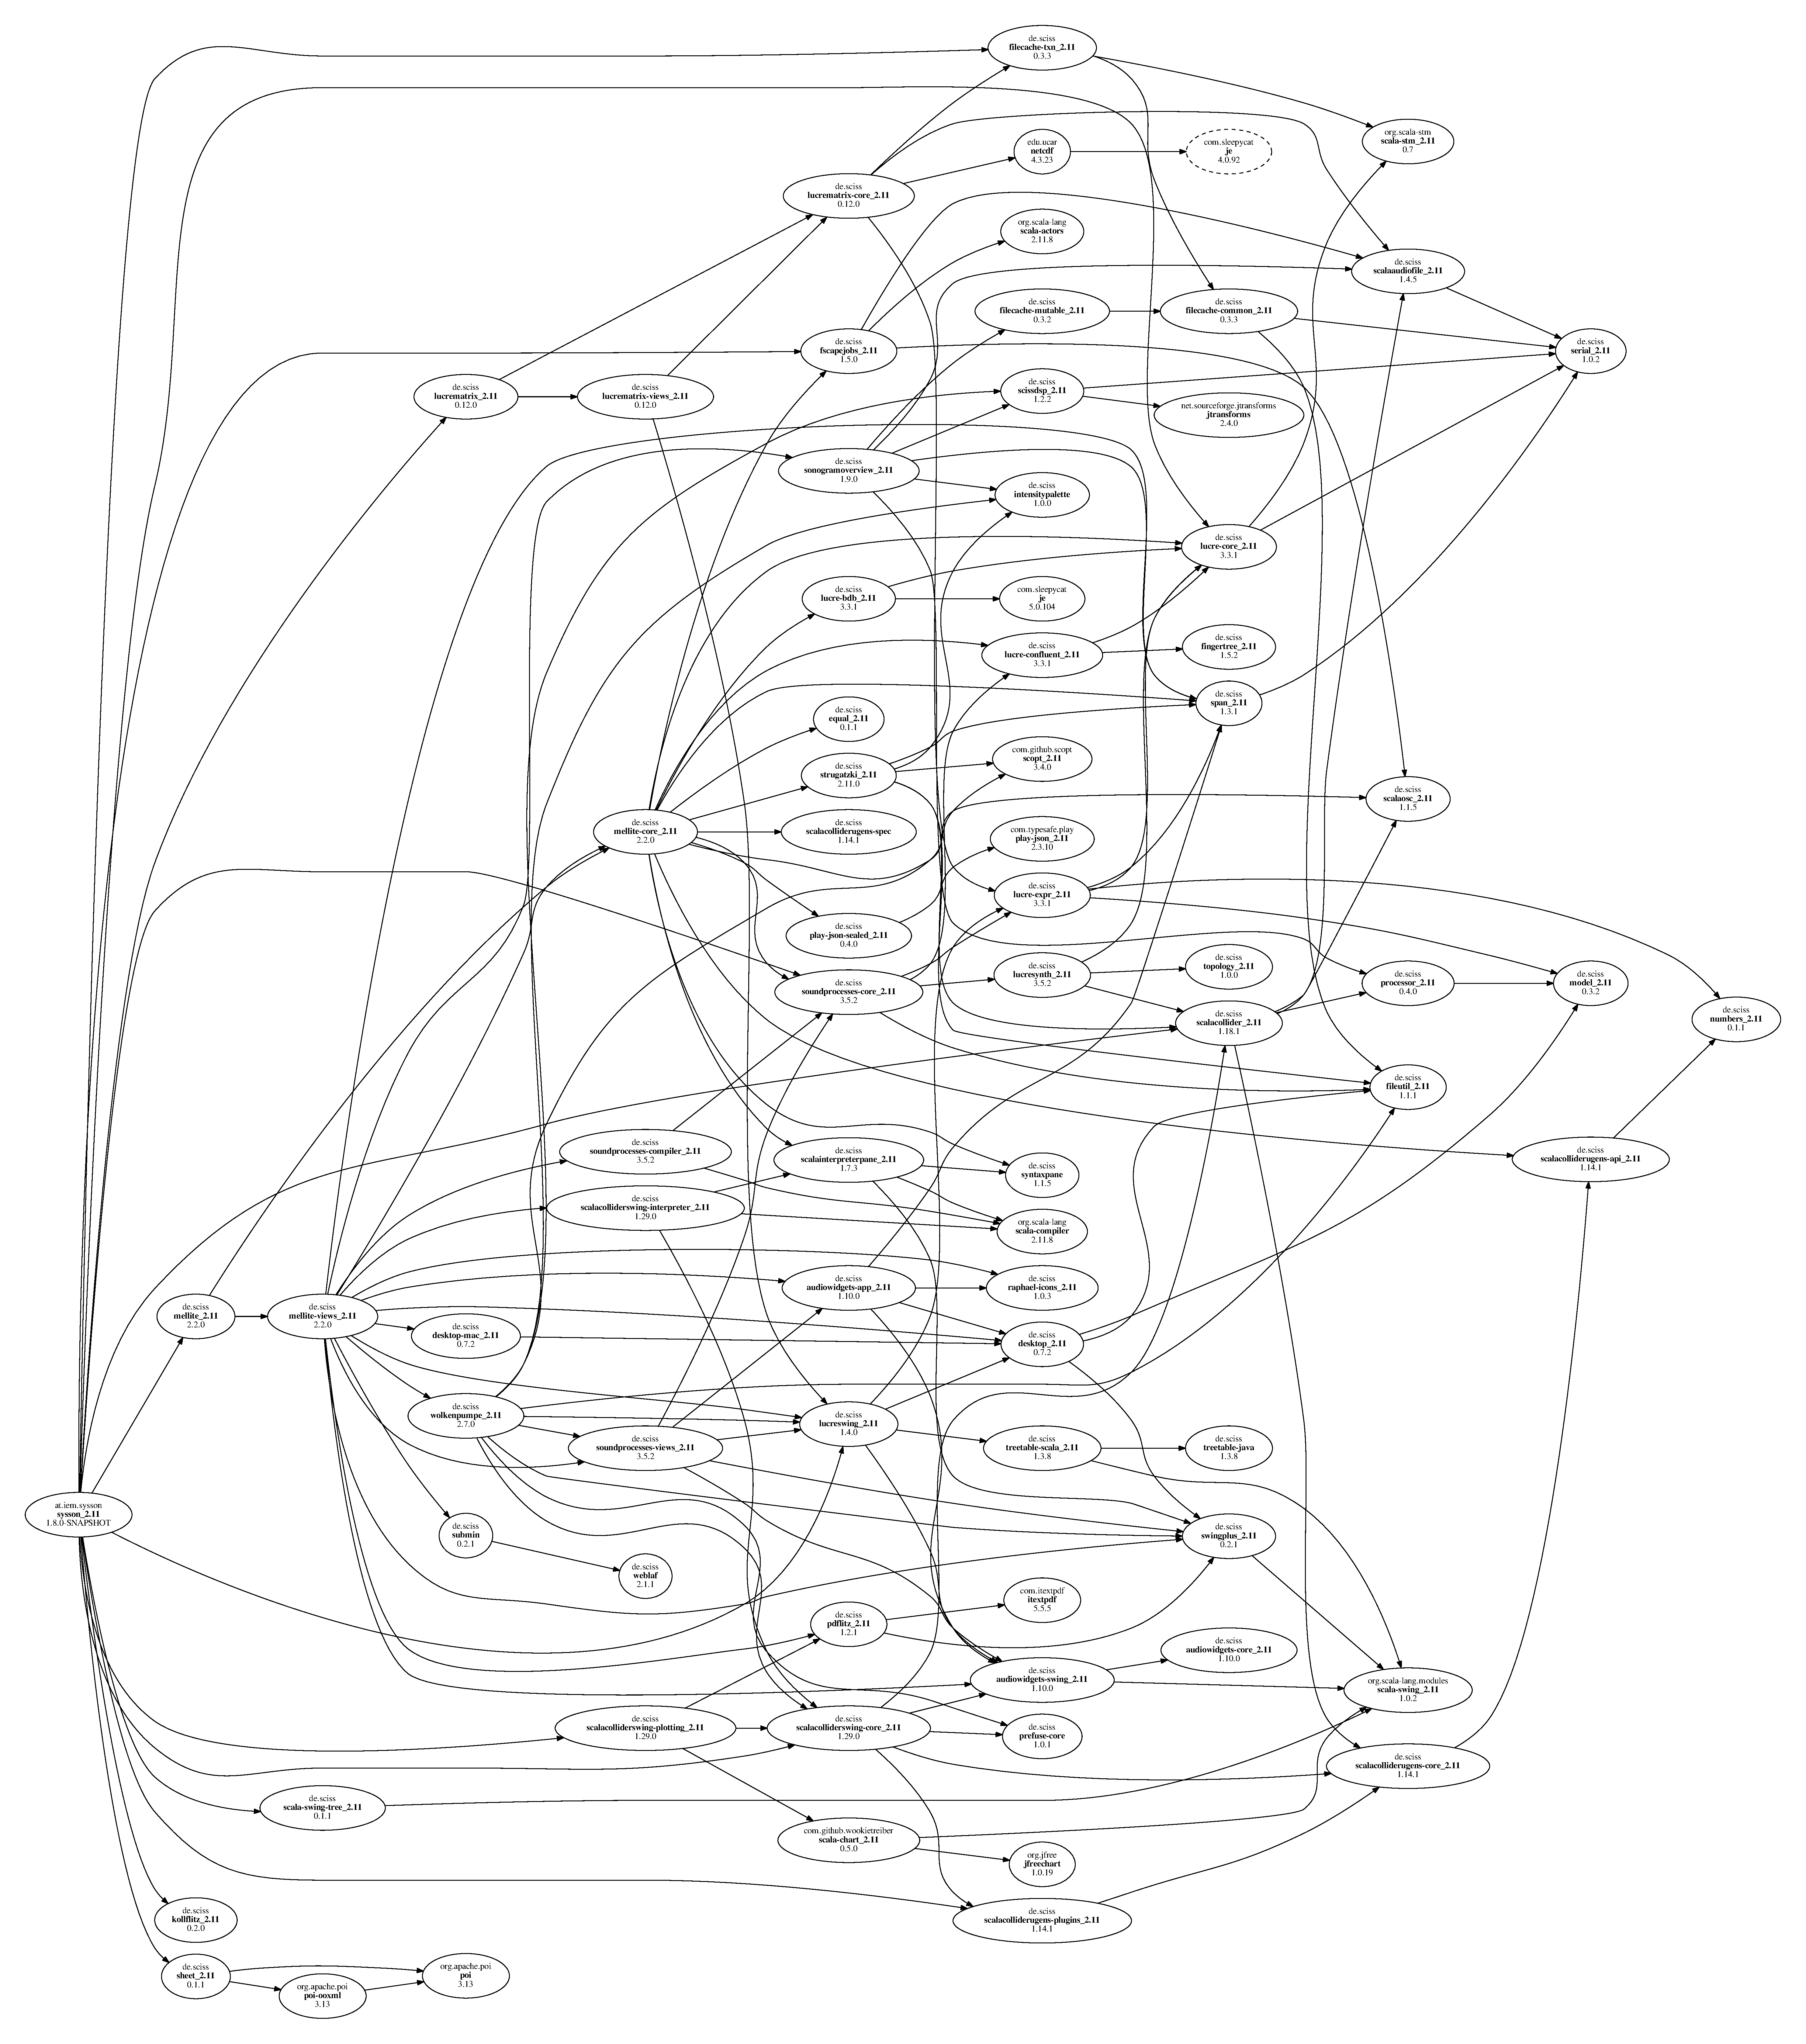
\includegraphics[width=\textwidth,trim=15mm 15mm 15mm 15mm]{figures/dependencies-compile.pdf}%
\caption{Module/library dependencies for SysSon version \syssonVersion{}}%
\label{fig:dependencies}%
\end{figure}

\end{document}
